\documentclass{standalone}
\usepackage{tikz}
\usepackage{ctex,siunitx,ninecolors}
\setCJKmainfont{Noto Serif CJK SC}
\usepackage{tkz-euclide}
\usepackage{amsmath}
\usetikzlibrary{patterns, calc}
\usetikzlibrary {decorations.pathmorphing, decorations.pathreplacing, decorations.shapes}
\begin{document}
\small
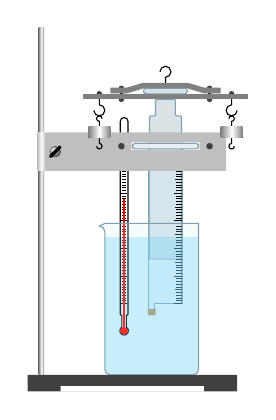
\begin{tikzpicture}[>=latex,scale=0.7]
  % \useasboundingbox(-1.4,-1.4)rectangle(1.4,1.4);
  \begin{scope}[xshift=-3mm,yshift=0.8cm]
    \fill[darkgray](-0.8,3.1)circle(0.05)(0.8,3.1)circle(0.05)(-0.8,2.9)circle(0.05)(0.8,2.9)circle(0.05)(1.2,3.0)circle(0.05)(-1.2,3.0)circle(0.05);
    \draw(-0.1,3.4)arc(180:-90:0.1)--++(0,-0.2);
    \draw(1.2,3)--++(0,-0.2)arc(90:360:0.1);
    \coordinate (A1) at (1.2,2.6);
    \draw(-1.2,3)--++(0,-0.2)arc(90:-180:0.1);
    \coordinate (B1) at (-1.2,2.6);
    \draw[very thick](-0.8,3.1)--(-0.8,2.9)(0.8,3.1)--(0.8,2.9);
    \fill[gray](-1.5,2.9)rectangle(1.5,3.0);
    \draw[gray,line width=0.7mm](-1.0,3.06)--(-0.7,3.06)--(-0.4,3.15)--(0.4,3.15)--(0.7,3.06)--(1.0,3.06);
    \draw[cyan!30!gray,fill=cyan!10!lightgray!50,rounded corners=0.14mm](-0.29,0)--(-0.29,2.6)--(-0.18,2.6)--(-0.18,2.9)--(0.18,2.9)--(0.18,2.6)--(0.29,2.6)--(0.29,0)--cycle;
    
    \draw[cyan!30!gray,fill=cyan!10!lightgray!50,rounded corners=0.35mm](-0.4,3.0)rectangle(0.4,3.1);
  \end{scope}
  \draw[cyan!30!gray,fill=cyan!20,fill opacity=0.3](0,0)--(-0.5,0)--(-0.5,-0.2)--(-0.6,-0.2)--(-0.6,2.8)--(0,2.8)--cycle;
  \draw[cyan!30!gray,fill=cyan!10!lightgray!30,rounded corners=0.35mm](-0.9,2.8)rectangle(0.3,2.9);
  \fill[brown,rounded corners=0.14mm](-0.62,-0.1)--(-0.62,-0.22)--(-0.48,-0.22)--(-0.48,-0.1);
  \foreach \y in {0,0.5,...,2.0}
  {
    \draw[ultra thin](0,\y)--++(-0.15,0);
    \draw[ultra thin](0,\y+0.25)--++(-0.12,0);
    \foreach \z in {1,2,3,4,6,7,8,9}
    {
      \draw[ultra thin](0,\y+0.05*\z)--++(-0.10,0);
    }
  }
  \draw[ultra thin](0,2.5)--++(-0.15,0);
  
  \fill[cyan!70!white,opacity=0.3](-1.4,1.2)--(-1.4,-1.2)arc(-180:-90:0.1)--(0.2,-1.3)arc(-90:0:0.1)--(0.3,1.2);
  \foreach \y in {0,0.5,...,2.5}
    {
      \draw[ultra thin](-1.1,\y)--++(0.1,0);
      \draw[ultra thin](-1.09,\y+0.25)--++(0.08,0);
      \foreach \z in {1,2,3,4,6,7,8,9}
      {
        \draw[ultra thin](-1.08,\y+0.05*\z)--++(0.06,0);
      }
    }
  \draw[ultra thin](-1.1,3.0)--++(0.1,0);
  \draw(-1.12,-0.2)--(-1.12,3.3)arc(180:0:0.07)--(-0.98,-0.2)arc(0:-90:0.03)--++(0,-0.2)arc(420:120:0.08)--++(0,0.2)arc(-90:-180:0.03);
  \fill[red](-1.05,-0.5)circle(0.07);
  \draw[thick,red](-1.05,-0.5)--++(0,2.4);
  \draw[cyan!30!gray,fill=cyan!20,fill opacity=0.2](-1.5,1.4)arc(90:0:0.1)--(-1.4,-1.2)arc(-180:-90:0.1)--(0.2,-1.3)arc(-90:0:0.1)--(0.3,1.45)--(-1.4,1.45)--cycle;

  \fill[lightgray,even odd rule](-2.48,2.4)rectangle(0.8,3.1)(-0.92,2.78)rectangle(0.32,2.92);
  \fill[darkgray](-1.1,2.85)circle(0.06)(0.5,2.85)circle(0.06);
  \fill[left color=gray,right color=gray,middle color=white](-2.5,-1.3)rectangle(-2.6,5.0);
  \fill[left color=lightgray,right color=lightgray,middle color=white](-2.48,2.4)rectangle(-2.62,3.1);
  \fill[ball color=lightgray](-2.3,2.75)circle(0.1);
  \draw[very thick,line cap=round]([shift=(-135:0.12)]-2.3,2.75)--++(45:0.24);
  \fill[darkgray,even odd rule](-2.8,-1.3)rectangle(1.0,-1.6)(-2.2,-1.5)rectangle(0.4,-1.6);

  \draw(B1)arc(90:0:0.05);
  \draw(B1)arc(90:270:0.05)--++(0,-0.4)arc(90:-180:0.05);
  \fill[left color=gray,right color=gray,middle color=white]([xshift=-2mm,yshift=-2mm]B1)rectangle++(0.4,-0.2);
  \draw(A1)arc(90:180:0.05);
  \draw(A1)arc(90:-90:0.05)--++(0,-0.4)arc(90:360:0.05);
  \fill[left color=gray,right color=gray,middle color=white]([xshift=-2mm,yshift=-2mm]A1)rectangle++(0.4,-0.2);
\end{tikzpicture}
\end{document}